The electronic system designed to perform a complete characterization of the SiPM S13360-6075 model, which is the one proposed for the final TRITIUM monitor is shown in this appendix. This system consists of three different PCBs connected through HDMI connectors:

\begin{enumerate}
\item{} In the first PCB, shown in Figure \ref{subfig:PCB1}, up to 8 SiPMs and one temperature sensor are connected. This PCB is placed inside a light-tight box from Thorlabs \cite{ThorlabsCompany}. This black box has a small hole of $1~\mm$ diameter, prepared to introduce an optical fiber\footnote{The optical fiber used is BCF-98 from Saint-Gobain \cite{OpticalFibers}} to illuminate SiPMs with a LED, model 430L from Thorlabs \cite{LEDThorlabs}. The spectrum of this LED, shown in Figure \ref{subfig:LEDSpectrum}, was measured with a spectrometer. The emission peak of this LED is located at $436~\nm$ with a FWHM of $19~\nano\meter$. With the help of this LED, the light emission of the TRITIUM scintillating fibers was simulated to calibrate the SiPMs at the working wavelength. 

\item{} In the second PCB, shown in Figure \ref{subfig:PCB2}, the signals of the SiPMs are summed and amplified by a factor either $G=4187$ or $G=10761$, depending on the input resistance of the oscilloscope, $50~\varOmega$ or $1~\mega\varOmega$ respectively. This PCB uses a differential amplifier to reduce the electronic noise of the system.

\item{} In the third PCB, shown in Figure \ref{subfig:PCB3}, the different input and output signals are rearranged to avoid crosstalk. The input signals are the supply voltage of the SiPMs and the PCBs ($\pm 6~\volt$) and the output signals are the temperature sensor signal and the sum of the SiPM signals. The output signal of the third PCB is connected to an oscilloscope, model MSO44X from Tektronix \cite{Oscilloscope}, that records the data.

\end{enumerate}

\begin{figure}
\centering
    \begin{subfigure}[b]{0.5\textwidth}
    \centering
    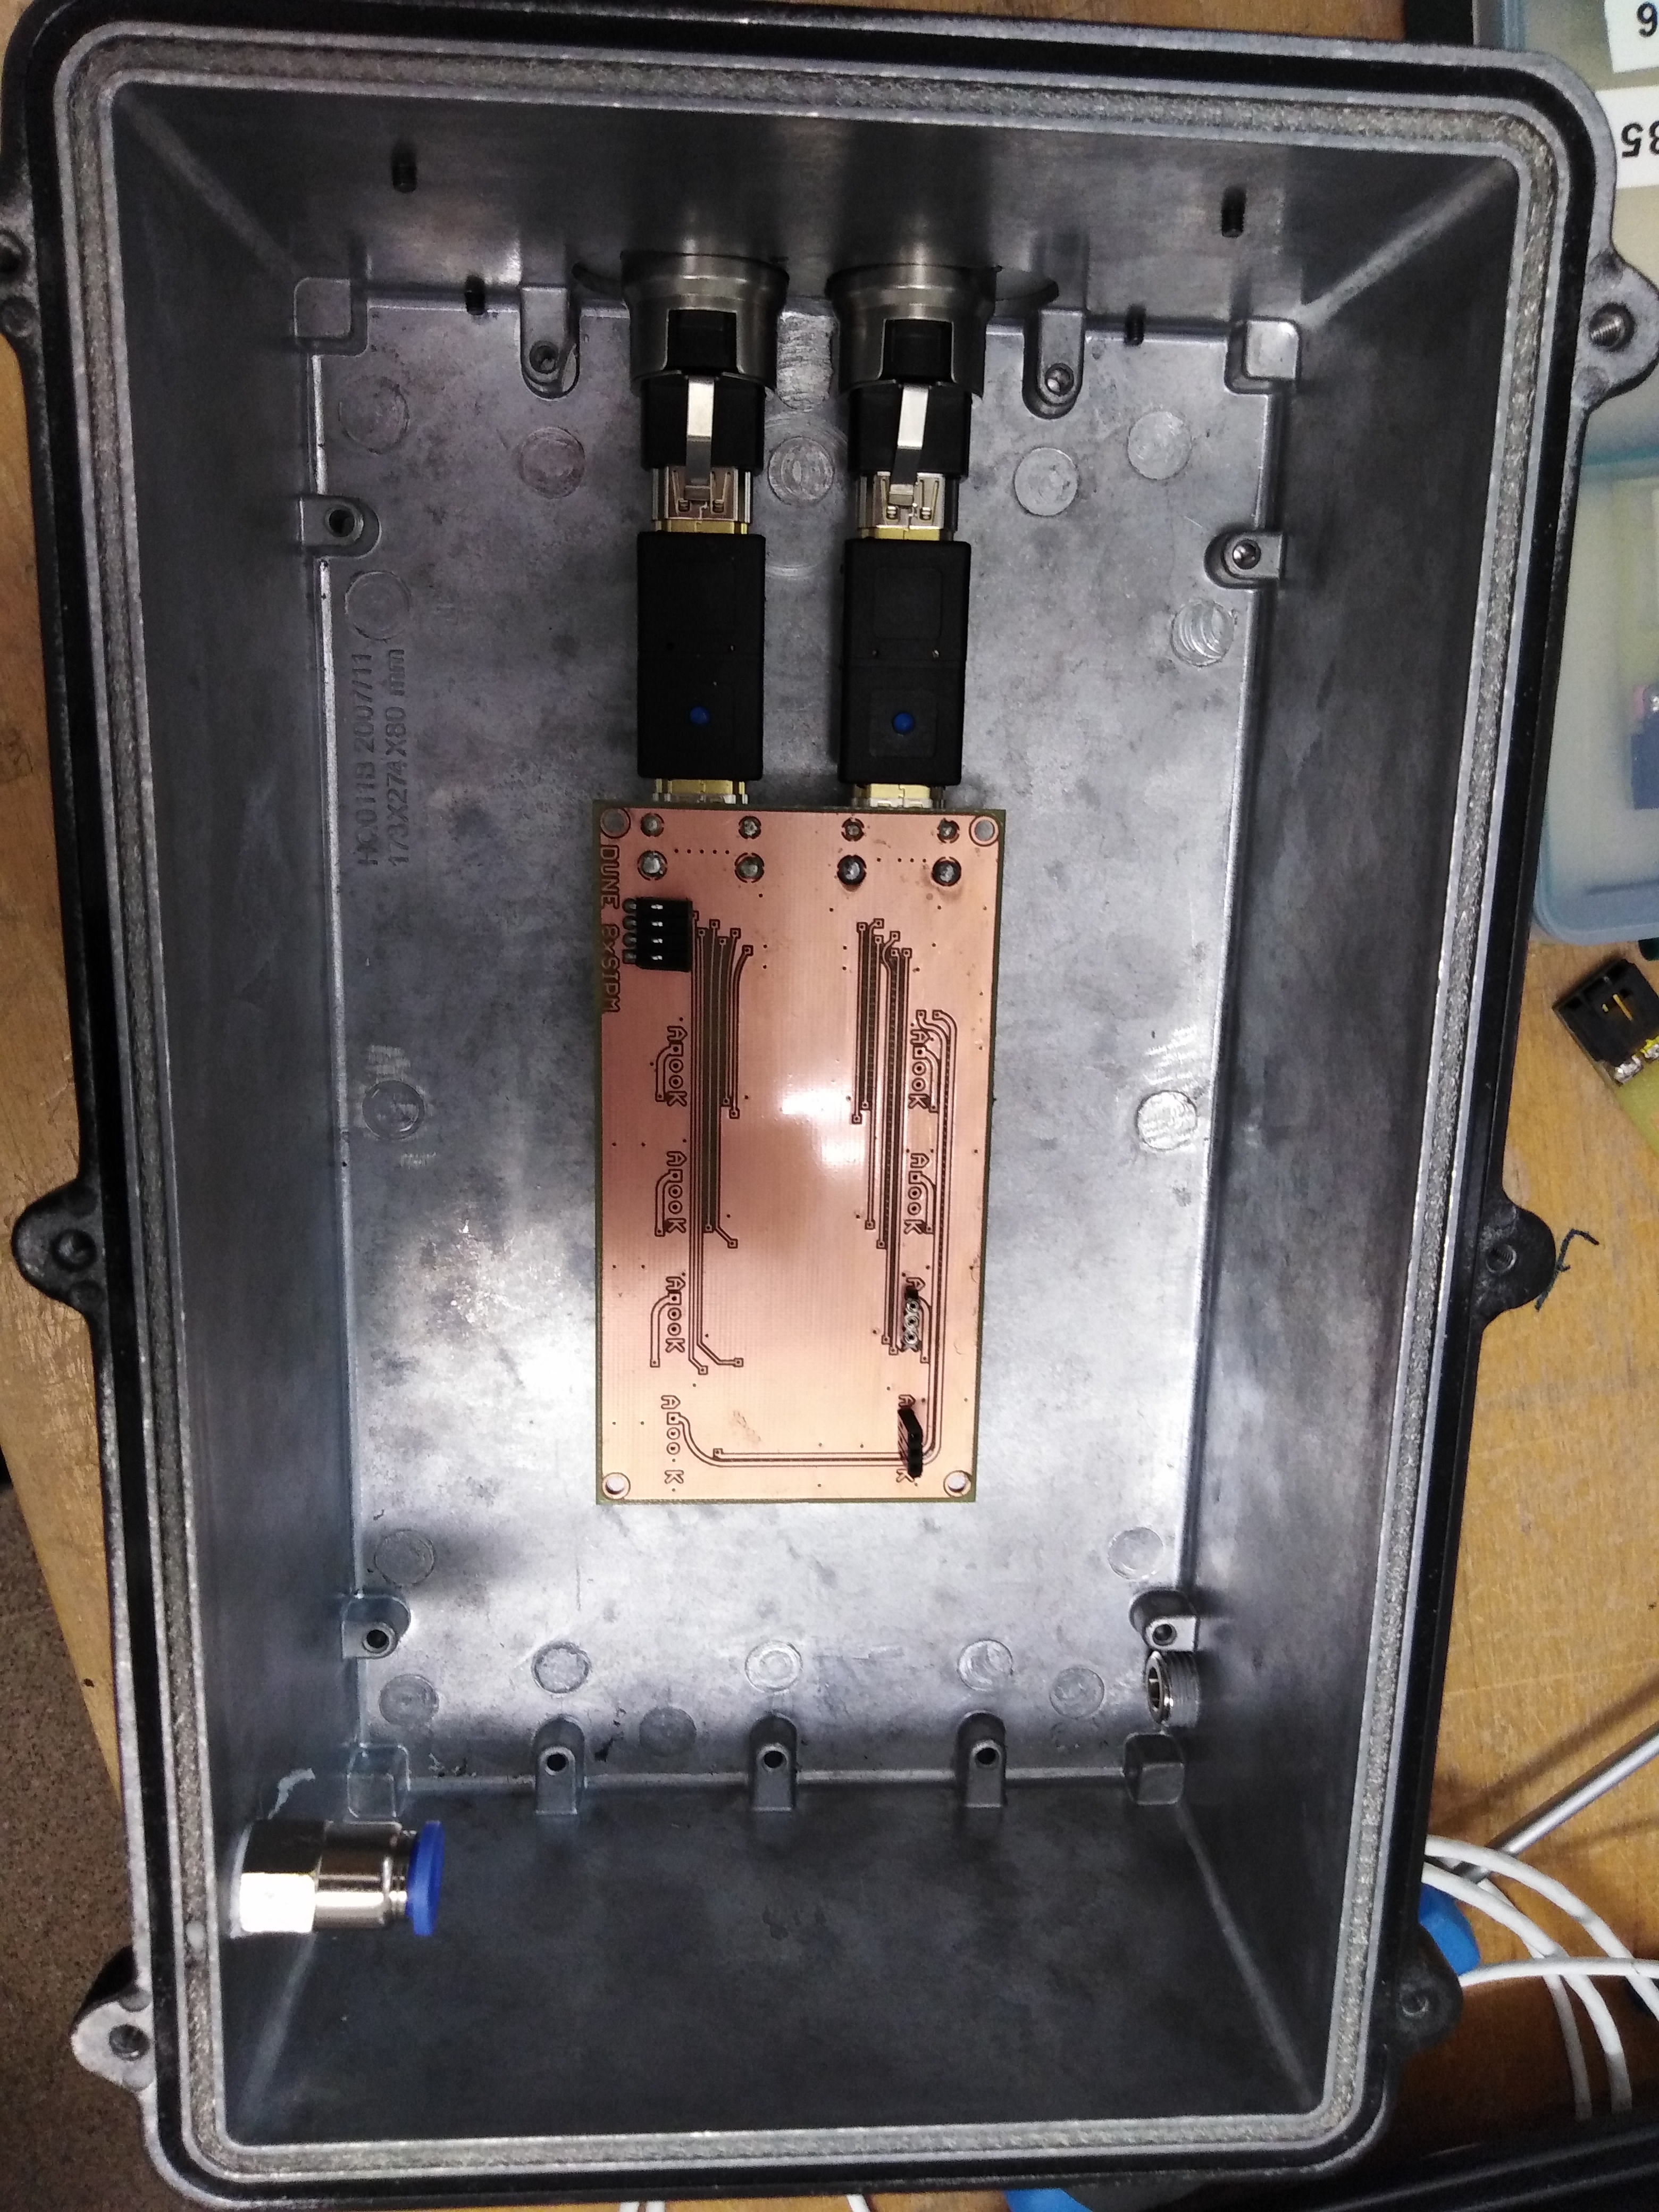
\includegraphics[width=\textwidth]{3DesignPrinciples/32Tritium_detector/PCB1_SiPM_Black_Box.jpg}  
    \caption{\label{subfig:PCB1}}
    \end{subfigure}
    \hfill
    \begin{subfigure}[b]{0.45\textwidth}
    \centering
    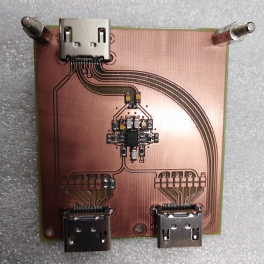
\includegraphics[width=\textwidth]{3DesignPrinciples/32Tritium_detector/PCB2_SIPMs.png}  
    \caption{\label{subfig:PCB2}}
    \end{subfigure}
    \hfill
    \begin{subfigure}[b]{0.4\textwidth}
    \centering
    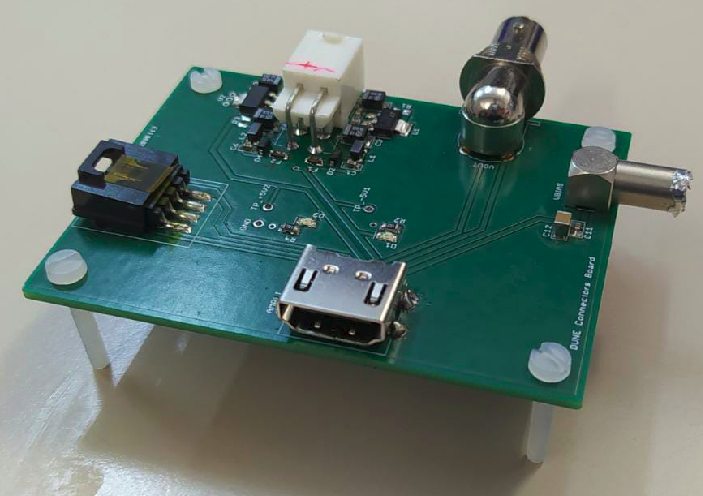
\includegraphics[width=\textwidth]{3DesignPrinciples/32Tritium_detector/PCB3_SiPMs.png}  
    \caption{\label{subfig:PCB3}}
    \end{subfigure}
    \hfill
    \begin{subfigure}[b]{0.5\textwidth}
    \centering
    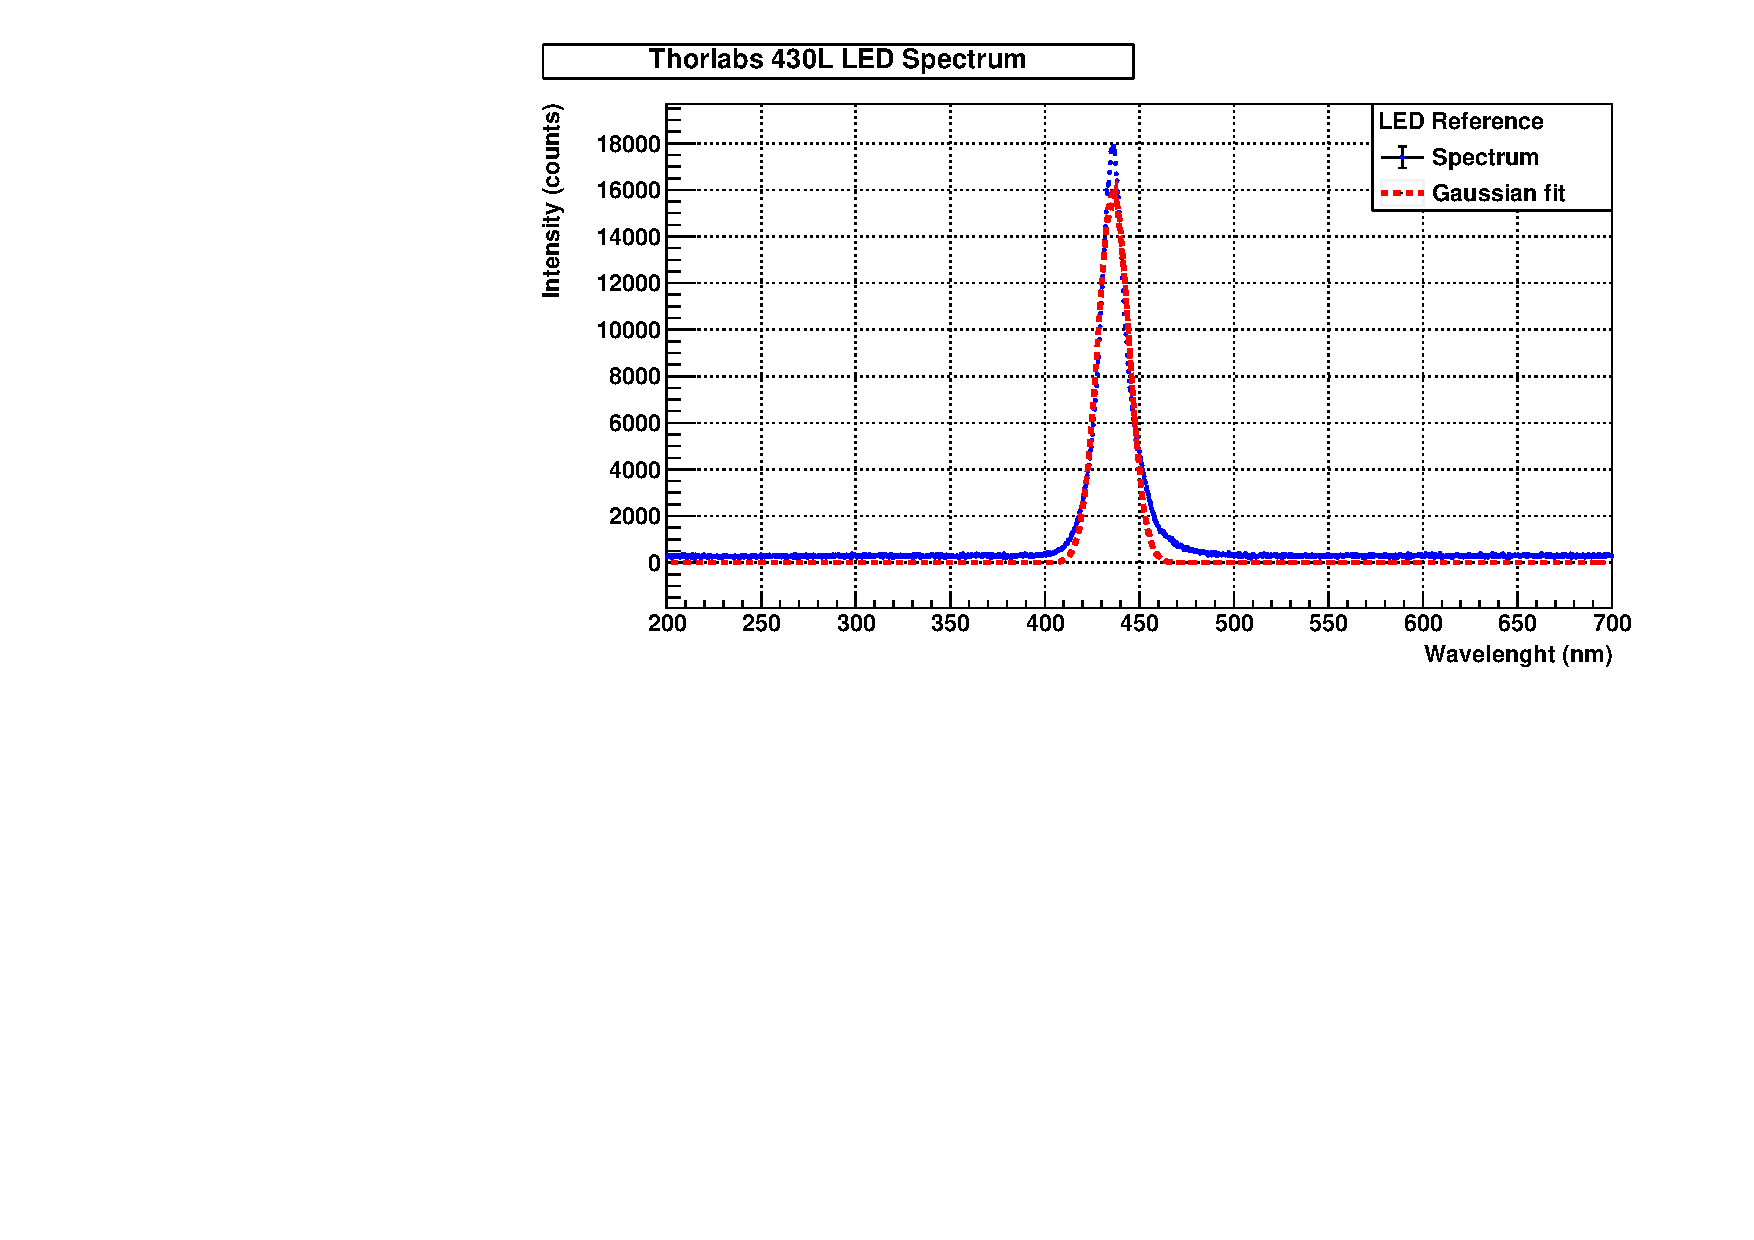
\includegraphics[width=\textwidth]{3DesignPrinciples/32Tritium_detector/LED_DUNE.pdf}  
    \caption{\label{subfig:LEDSpectrum}}
    \end{subfigure}
 \caption{The three PCBs used for SiPM characterization a) The PCB 1 used to connect up to 8 SiPMs inside the black box. b) The PCB 2 used to sum and amplify the output signals of the SiPMs. c) The PCB 3 used to rearrange the input and output signals of the system. d) The LED emission spectrum.}
 \label{fig:PCBs_LEDSpectrum}
\end{figure}